\documentclass[a4paper]{article}
\usepackage{calc,amsmath,amssymb,amsfonts}
\usepackage[T2A,LGR,T1]{fontenc}
\usepackage[greek,english,russian]{babel}
\usepackage{xcolor,longfbox,fancyhdr}
\usepackage[top=0.7874in,bottom=0.1028in,left=1.1811in,right=0.5902in,nohead,includefoot,foot=0.6846in,footskip=1.3299in]{geometry}
\usepackage{enumitem,hyperref}
\hypersetup{colorlinks=true,allcolors=blue,pdfauthor=Misha Sedov}
\usepackage[pdftex]{graphicx}
\usepackage{tikz}
\makeatletter\newdimen\@tempdimd\makeatother
% Outline numbering
\setcounter{secnumdepth}{0}
% Text styles
\newcommand\textstyleHTMLCode[1]{\textrm{#1}}
% Pages
\fancypagestyle{Standard}{\fancyhf{}
  \fancyhead[L]{}
  \fancyfoot[C]{\thepage{}}
  \renewcommand\headrulewidth{0pt}
  \renewcommand\footrulewidth{0pt}
  \renewcommand\thepage{\arabic{page}}
}
\fancypagestyle{FirstPage}{\fancyhf{}
  \fancyhead[L]{}
  \fancyfoot[L]{}
  \renewcommand\headrulewidth{0pt}
  \renewcommand\footrulewidth{0pt}
  \renewcommand\thepage{\arabic{page}}
}
\pagestyle{Standard}
\newcounter{qwerty}
\renewcommand\theqwerty{\arabic{qwerty}}
\author{Misha Sedov}
\date{2023-05-26}
\begin{document}
\clearpage
\pagestyle{Standard}
\thispagestyle{FirstPage}
{\centering
Министерство образования и науки Российской Федерации
\par}

{\centering

Московский авиационный институт (национальный исследовательский университет)

\par}

{\centering
г. Москвы
\par}

{\centering
$\text{\textgreek{«}}$МАИ\text{\textgreek{»}}$
\par}


\bigskip


\bigskip


\bigskip


\bigskip


\bigskip


\bigskip


\bigskip

{\centering
$\text{\textgreek{«}}$\MakeUppercase{Создание и внедрение роботизированной платформы автономного позиционирования и
навигации}$\text{\textgreek{»}}$
\par}


\bigskip


\bigskip


\bigskip

{\raggedleft
Автор Седов Михаил Артёмович
\par}

{\raggedleft
Группа: М8О-116БВ-24 
\par}

{\raggedleft
Руководитель Крылов Евгений Евгеньевич
\par}

{\raggedleft
Инженер внедрения ООО $\text{\textgreek{«}}$Цифровая индустриальная платформа$\text{\textgreek{»}}$
\par}


\bigskip


\bigskip


\bigskip

{\centering
Г. Москва
\par}

{\centering
2024–2025 учебный год
\par}

\clearpage{\centering
СОДЕРЖАНИЕ
\par}

\setcounter{tocdepth}{10}
\tableofcontents
\section{ВВЕДЕНИЕ}
\subsection[Актуальность]{Актуальност\foreignlanguage{english}{1}ь}
Умные носилки должны будут выполнять часть функций медперсонала: перевозку больных по медицинским заведениям, помощь
посетителям в ориентировании по медицинским учреждениям. Ориентироваться по сооружениям они будут по встроенным в них
гироскопам, картам, камере, помогающей объезжать людей.

\subsection{Объект}
Роботизированная платформа автономного позиционирования и навигации под управление \foreignlanguage{english}{Robotic}
\foreignlanguage{english}{Operating} \foreignlanguage{english}{System} (\foreignlanguage{english}{ROS}) на базе
микрокомпьютера Raspberry \foreignlanguage{english}{Pi}.

\subsection{Предмет}
Работа алгоритма \foreignlanguage{english}{SLAM} (одновременное позиционирование и построение карты местности); работа
лидара; Взаимодействие платы микрокомпьютера и подключенных устройств; основы программирования для
\foreignlanguage{english}{ROS}; организация удалённого взаимодействия управляющего ПК с Ubuntu и робота с
\foreignlanguage{english}{ROS}

\subsection{Цель работы}
Сборка, программирование и тестирование робота, созданного на базе Raspberry Pi, с помощью
\foreignlanguage{english}{ROS} и Ubuntu.

\subsection{Задачи}
\begin{enumerate}[series=listWWNumxxiii,label=\arabic*),ref=\arabic*]
\item Сборка:

\begin{enumerate}[series=listWWNumxxiii,label=\alph*),ref=\alph*]
\item Электрические соединения:

\begin{enumerate}[series=listWWNumxxiii,label=\roman*),ref=\roman*]
\item Электродвигатели, 2 шт.
\item Плата контролеров + гироскоп
\item Raspberry Pi
\item Лидар
\item Дисплей
\item Видеокамера
\item Аккумулятор 
\end{enumerate}
\item Механические узлы

\begin{enumerate}[resume*=listWWNumxxiii,start=1]
\item Шасси
\item Зубчатые и опорные колёса
\item Гусеницы
\item Крепёж для электрических узлов
\end{enumerate}
\end{enumerate}
\item Программирование

\begin{enumerate}[resume*=listWWNumxxiii,start=1]
\item \begin{enumerate}[resume*=listWWNumxxiii,start=1]
\item Инициализация операционных систем Raspbian и ROS на плате Raspberry Pi.
\item Развёртывание операционной системы Ubuntu 16на ПК
\item Развёртывание операционной системы ROS и утилит для сборки программного кода робота в среде Ubuntu
\item Компиляция кода робота и перенос кода на Raspberry Pi
\item Соединение операционных систем ROS между ПК и Raspberry Pi посредством протокола SSH
\end{enumerate}
\end{enumerate}
\item Тестирование

\begin{enumerate}[resume*=listWWNumxxiii,start=1]
\item \begin{enumerate}[resume*=listWWNumxxiii,start=1]
\item Тестирование кода робота в эмуляторе под Ubuntu
\item Инициализация ROS на роботе по средствам SSH
\item Калибровка гироскопа
\item Построение и сохранение карты местности в памяти робота с помощью лидара и ручного управления движением робота
\item Запуск на роботе команд автономной навигации по заданным точкам на карте с объездом ненанесённых на карту
препятствий
\end{enumerate}
\end{enumerate}
\end{enumerate}

\bigskip

\section[Описание ROS 1]{Описание \foreignlanguage{english}{ROS} 1}
ROS (Robot Operation System) $\text{\textgreek{—}}$ это операционная система для роботов. Она обеспечивает всю
необходимую функциональность для распределённой работы всех узлов робота. На самом деле ROS $\text{\textgreek{—}}$ это
библиотека, надстройка поверх компьютерной операционной системы. ROS предоставляет стандартные возможности операционной
системы, такие как аппаратная абстракция, низкоуровневое управление устройствами, реализация часто используемых
функций, передача сообщений между процессами и управление пакетами.

ROS содержит множество пакетов для создания виртуального робота и симулирования его поведения $\text{\textgreek{—}}$
например, стек пакетов gazebo\_ros\_pkgs. C помощью Gazebo вы сможете даже симулировать знаменитого робота Atlas от
Boston Dynamics у себя на компьютере.

\section{Дифференциальный привод с гусеницами}
Дифференциальный привод с гусеницами (танковое шасси) $\text{\textgreek{—}}$ версия привода skid-steer с гусеницами
вместо дополнительных колёс. Каждая гусеница и сторона робота контролируется одним мотором.

Можно интерпретировать этот привод как двухколёсный дифференциальный, где колесо имеет некруглую форму и увеличенную
длину окружности (Рисунок 1). Или как привод skid-steer с бесконечным количеством колёс на определённой длине.
\lfbox[margin-right=0.0035in,margin-top=0mm,margin-bottom=0mm,margin-left=0mm,border-style=none,padding=0mm,vertical-align=top]{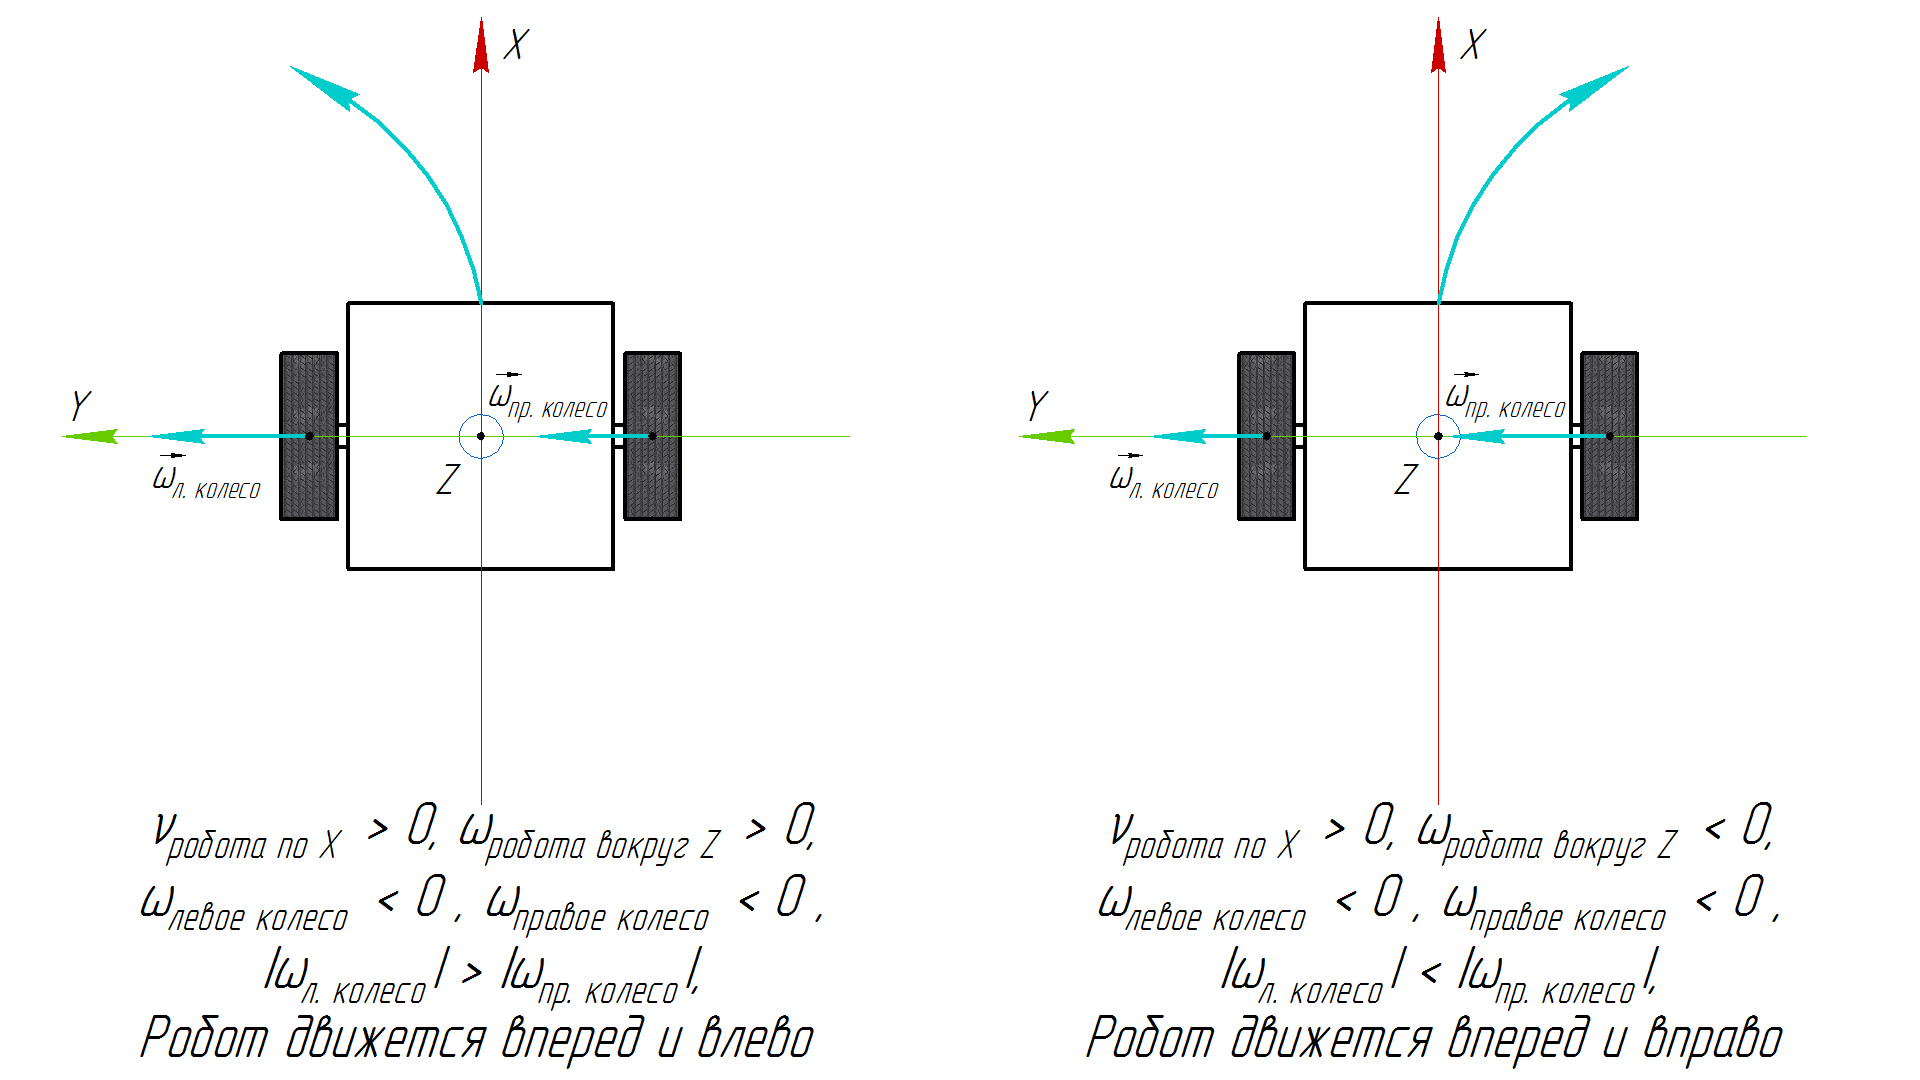
\includegraphics[width=6.4965in,height=3.6543in]{a0000-img001.png}}


{\centering\itshape\color[HTML]{44546A}
\label{bkm:Ref127517653}Рисунок \stepcounter{qwerty}{\theqwerty}. Принцип действия дифференциального привада с двумя
колёсами (гусеницами)
\par}

Движение привода с гусеницами неголономно. Принцип движения тут такой же, как и у привода skid-steer. Только для
обработки перемещения робота используются не угловые скорости колёс, а скорости гусениц.

Особенности шасси:

•\ \ Танковое шасси обладает самыми высокими эксплуатационными характеристиками на пересечённой местности благодаря
форме гусениц и сцеплению с землёй.

•\ \ Усложнённая механика. В конструкции танкового шасси множество непростых деталей: части трака, натяжители, опорные
ролики и т. д.

•\ \ Получить одометрию ещё сложнее, чем при использовании привода skid-steer. При движении танкового шасси тоже
происходят проскальзывания гусениц и заносы (особенно это заметно, когда робот-танк вращается на месте на ровной
поверхности). Однако ввиду наличия всего двух датчиков вращения программно компенсировать ошибки одометрии очень
тяжело. При движении по ровной поверхности одометрия неточная, а на пересечённой местности датчики вращения становятся
практически бесполезны, и для одометрии понадобятся другие источники.

\section{Теория навигации}
Автономная навигация робота строится на трёх фундаментальных принципах:

\begin{enumerate}[series=listWWNumiii,label=\arabic*.,ref=\arabic*]
\item Построение карт $\text{\textgreek{—}}$ Mapping.
\item Локализация в пространстве $\text{\textgreek{—}}$ Localization.
\item Планирование пути $\text{\textgreek{—}}$ Path planning.
\end{enumerate}
Их задачи:

\begin{enumerate}[series=listWWNumiv,label=\arabic*.,ref=\arabic*]
\item Задача маппинга состоит в том, чтобы ответить на вопрос робота: $\text{\textgreek{«}}$Как выглядит окружающее меня
пространство?$\text{\textgreek{»}}$ Во время картографирования данные с различных датчиков передаются роботу. На основе
этих данных робот строит карту окружающего мира (map) в понятном для себя представлении $\text{\textgreek{—}}$
топологическом или метрическом.
\item Задача локализации состоит в том, чтобы ответить на вопрос робота: $\text{\textgreek{«}}$Где я нахожусь в
окружающем меня мире?$\text{\textgreek{»}}$ Во время локализации робот определяет своё положение относительно карты
(map), которая может быть уже известна роботу или строиться в режиме реального времени. При локализации на заранее
известной карте робот должен уметь определять своё положение, где бы он не находился.
\item Задача планирования пути состоит в том, чтобы ответить на вопрос робота: $\text{\textgreek{«}}$Как я могу
добраться до определённой точки на карте?$\text{\textgreek{»}}$ Целевая точка на карте может быть установлена
оператором робота или самим роботом. Он должен уметь cамостоятельно прокладывать траекторию движения к целевой точке на
карте и добираться до этой точки. Кроме этого, траектория движения должна быть оптимальна и безопасна для робота.
\end{enumerate}
Различные комбинации этих трёх процессов позволяют мобильному роботу решать разнообразные навигационные задачи (Рисунок
2):

.\textcolor{black}{ }
\lfbox[margin-right=0.0035in,margin-top=0mm,margin-bottom=0mm,margin-left=0mm,border-style=none,padding=0mm,vertical-align=top]{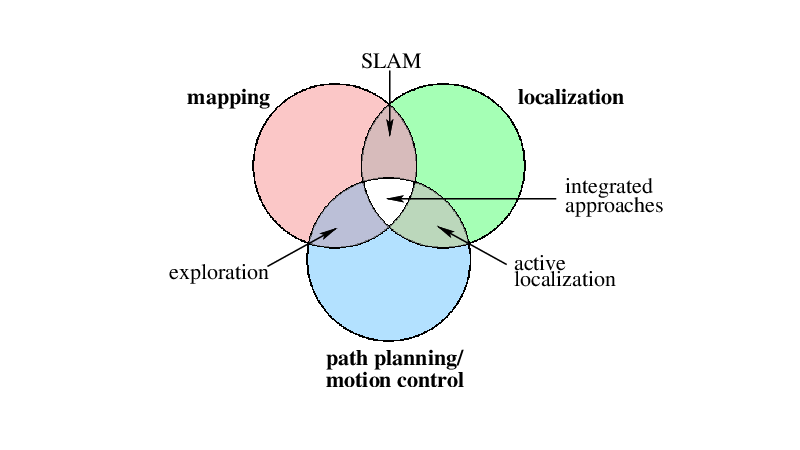
\includegraphics[width=6.4965in,height=3.6543in]{a0000-img002.png}}


{\centering\itshape\color[HTML]{44546A}
\label{bkm:Ref127518730}Рисунок \stepcounter{qwerty}{\theqwerty}. Принцип действия трёх процессов: маппинга локализации
планирования пути \ 
\par}

Что из всего этого будем использовать мы? Для начала мы составим методом SLAM глобальную карту помещения, где будет
работать наш робот.

Затем мы дадим роботу эту карту помещения и будем управлять им, задавая целевые точки (Goal points) на ней. До этих
точек робот должен будет добираться самостоятельно, объезжая все препятствия на пути и при этом не теряя себя на карте.
Таким образом, мы будем использовать метод Active localisation.

\section{Лидар}
Такой датчик способен отсканировать всю плоскость, в которой он установлен. Почему именно лидар? Потому что этот тип
датчиков настолько эффективен, что одного устройства может быть достаточно для реализации навигации в помещении!


\lfbox[margin-right=0.0035in,margin-bottom=0.0102in,margin-top=0mm,margin-left=0mm,border-style=none,padding=0mm,vertical-align=top]{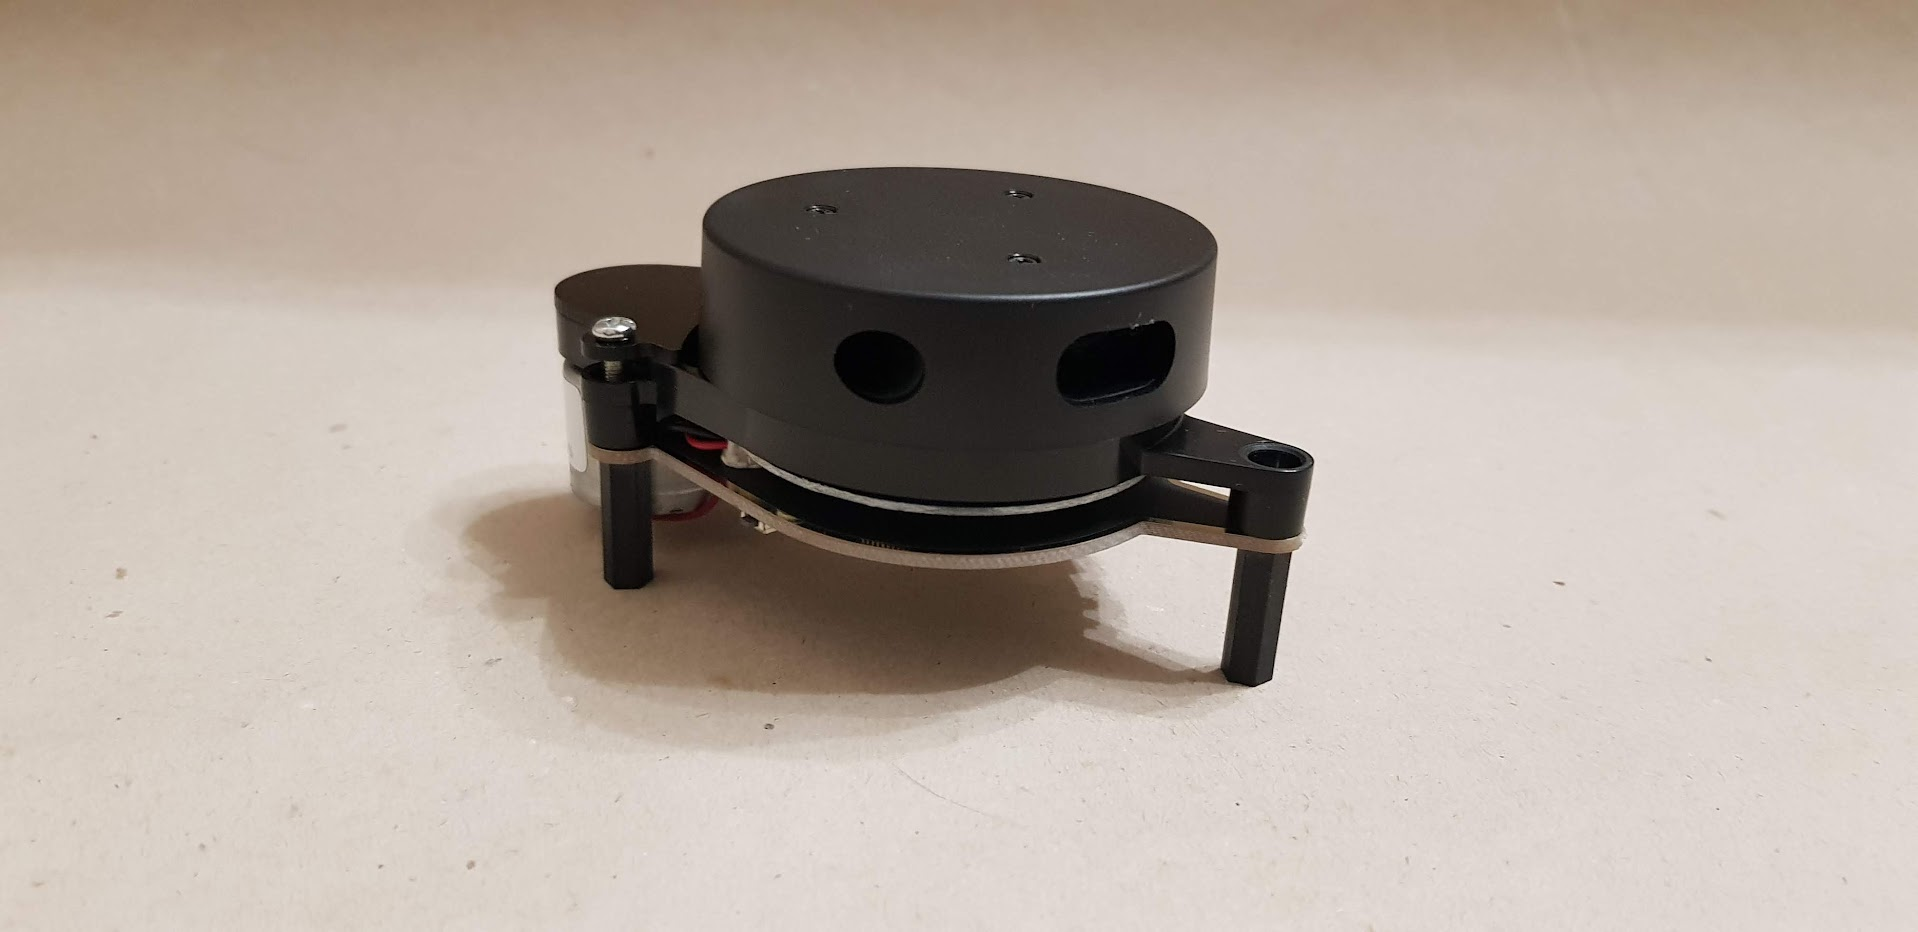
\includegraphics[width=6.4965in,height=3.1563in]{a0000-img003.jpg}}


{\centering\itshape\color[HTML]{44546A}
Рисунок \stepcounter{qwerty}{\theqwerty}. Лидар
\par}

\section{Сборка}
\centering
\lfbox[margin-right=0.0035in,margin-bottom=0.002in,margin-top=0mm,margin-left=0mm,border-style=none,padding=0mm,vertical-align=top]{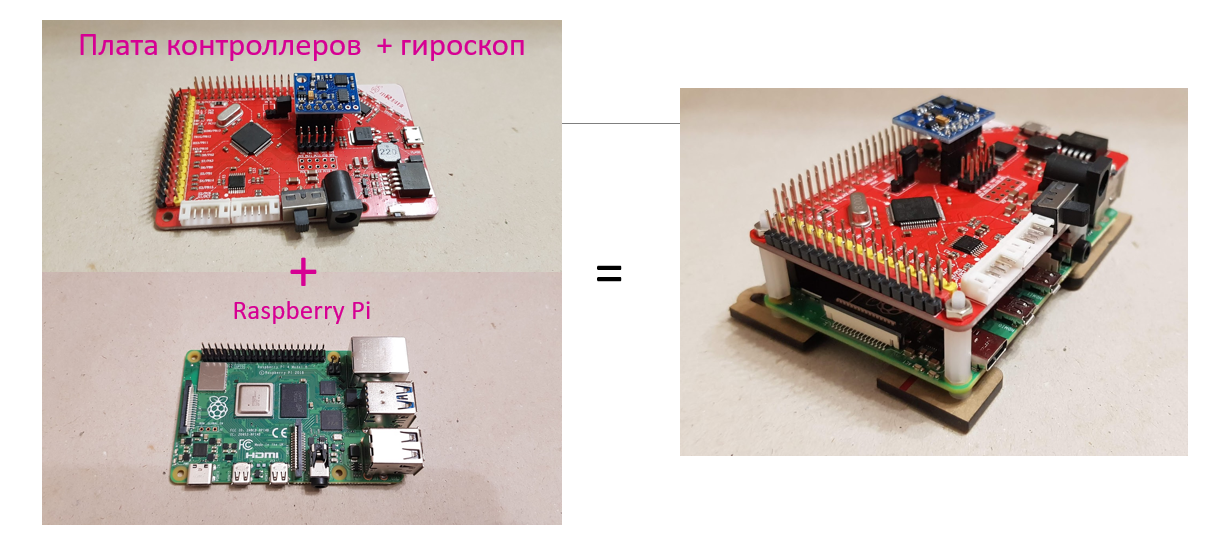
\includegraphics[width=6.4965in,height=2.8728in]{a0000-img004.png}}
\par
{\centering\itshape\color[HTML]{44546A}
Рисунок \stepcounter{qwerty}{\theqwerty}. Подключение платы контролера к Raspberry Pi
\par}

\centering
\lfbox[margin-right=0.0035in,margin-bottom=0.0102in,margin-top=0mm,margin-left=0mm,border-style=none,padding=0mm,vertical-align=top]{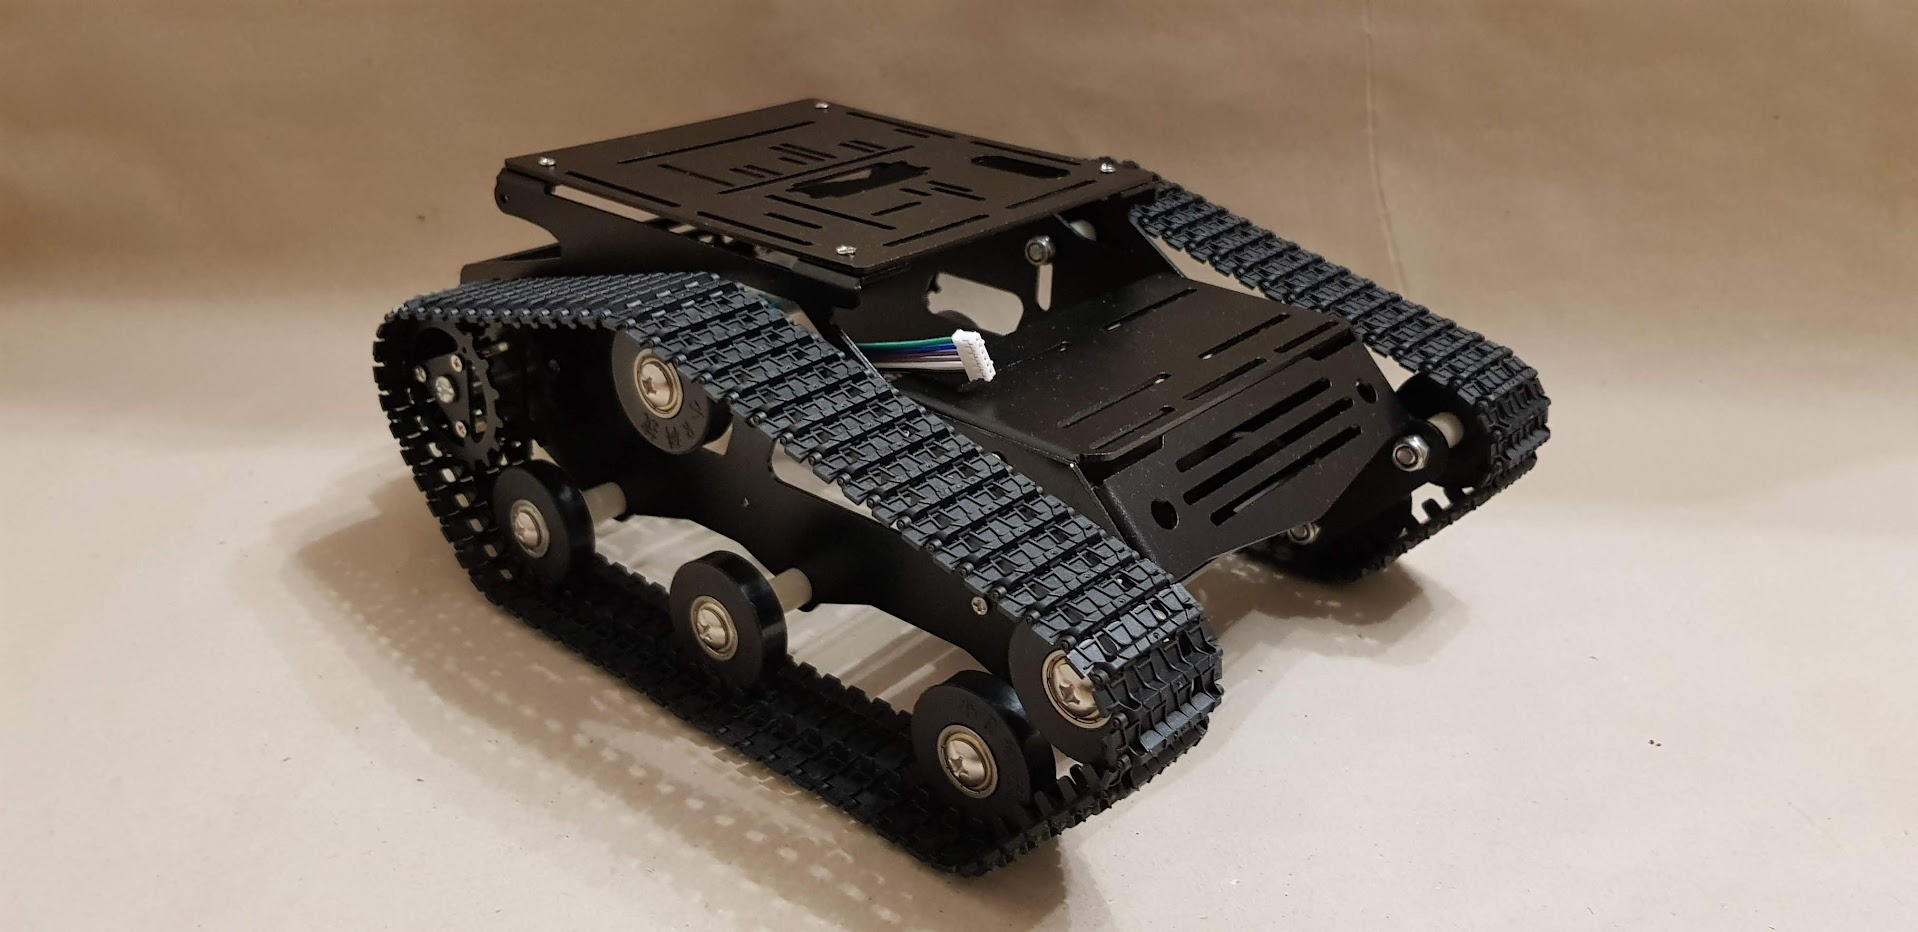
\includegraphics[width=6.4965in,height=3.1563in]{a0000-img005.jpg}}
\par
{\centering\itshape\color[HTML]{44546A}
Рисунок \stepcounter{qwerty}{\theqwerty}. Шасси в сборе
\par}


\bigskip

\centering
\lfbox[margin-bottom=0.0102in,margin-top=0mm,margin-right=0mm,margin-left=0mm,border-style=none,padding=0mm,vertical-align=top]{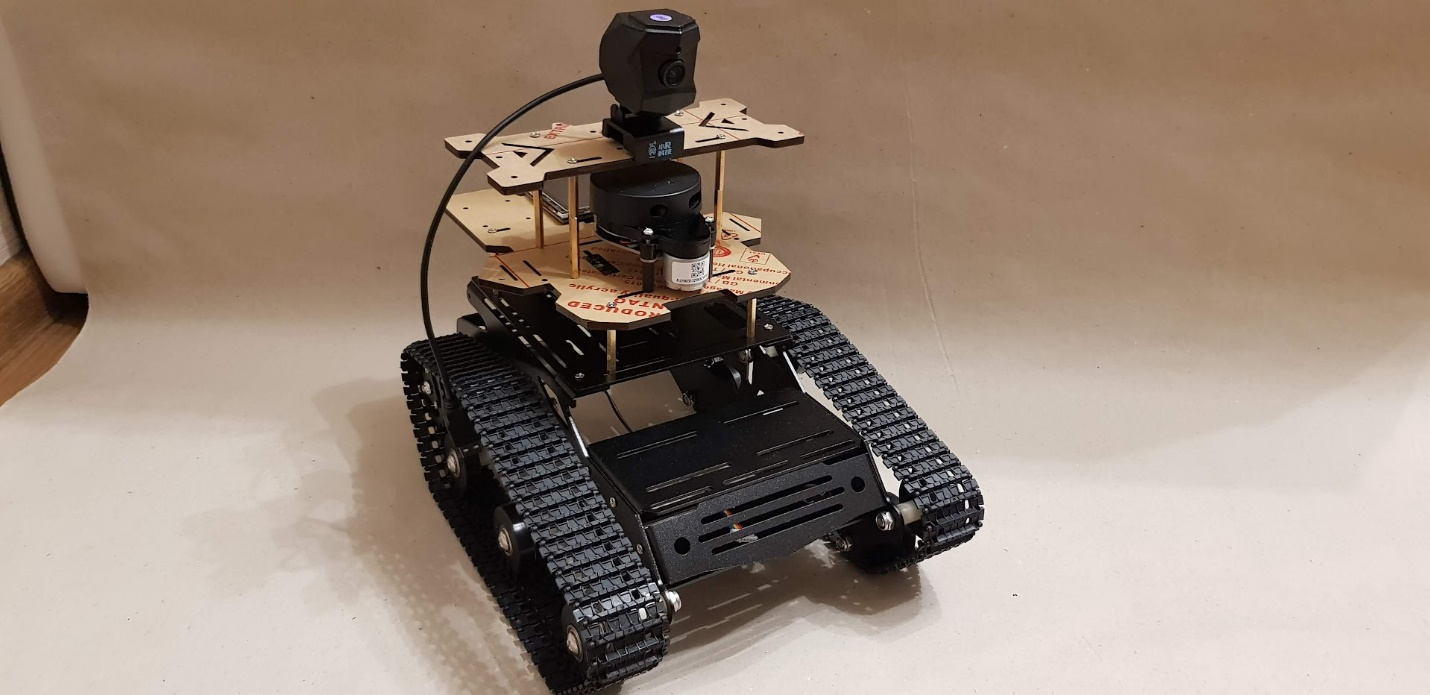
\includegraphics[width=4.8752in,height=3.1563in]{a0000-img006.jpg}}
\par
{\centering\itshape\color[HTML]{44546A}
Рисунок \stepcounter{qwerty}{\theqwerty}. Робот в сборе
\par}


\bigskip


\bigskip


\bigskip

\section{Программирование}
Развернул виртуальную машину \foreignlanguage{english}{VMware} с операционной системой \foreignlanguage{english}{Ubuntu}
16.04.

\centering
\lfbox[margin=0mm,border-style=none,padding-top=0.0492in,padding-right=0.0984in,padding-bottom=0.0492in,padding-left=0.0984in]{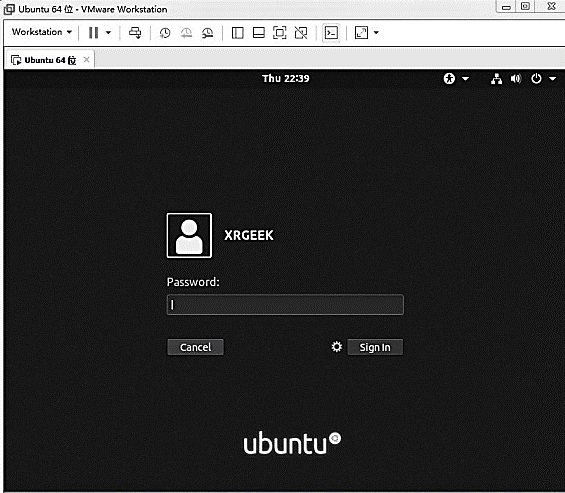
\includegraphics[width=4.7087in,height=3.5189in]{a0000-img007.png}}
\par
{\centering\itshape\color[HTML]{44546A}
Рисунок \stepcounter{qwerty}{\theqwerty}. Вход в \foreignlanguage{english}{Ubuntu}
\par}

Развернул операционную систему \foreignlanguage{english}{ROS} \foreignlanguage{english}{Kinetic} с помощью команды

\textstyleHTMLCode{\foreignlanguage{english}{sudo apt-get install ros-kinetic-full}}

Выполнил сборку кода робота с помощью утилиты \foreignlanguage{english}{catkin}\_\foreignlanguage{english}{make}

\textstyleHTMLCode{\foreignlanguage{english}{catkin\_make}}

\textstyleHTMLCode{\foreignlanguage{english}{source devel/setup .bash}}

Перенёс готовый код на карту памяти робота 

Подключился по \foreignlanguage{english}{SSH} к роботу

\textstyleHTMLCode{ssh xrrobot@192.168.1.1}

Инициализировал операционную систему \foreignlanguage{english}{ROS} командой 

\textstyleHTMLCode{\foreignlanguage{english}{r}oscore}

\centering
\lfbox[margin=0mm,border-style=none,padding-top=0.0492in,padding-right=0.0984in,padding-bottom=0.0492in,padding-left=0.0984in]{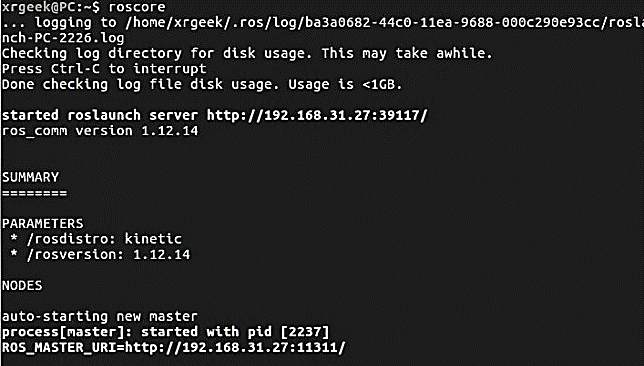
\includegraphics[width=5.3677in,height=3.0512in]{a0000-img008.png}}
\par
{\centering\itshape\color[HTML]{44546A}
Рисунок \stepcounter{qwerty}{\theqwerty}. Инициализация \foreignlanguage{english}{ROS}
\par}


\bigskip

\section{Тестирование}
\begin{enumerate}[series=listWWNumxvii,label=\arabic*.,ref=\arabic*]
\item Подключился по \foreignlanguage{english}{SSH} к роботу
\end{enumerate}
\textstyleHTMLCode{ssh xrrobot@192.168.1.1}

\begin{enumerate}[resume*=listWWNumxvii]
\item Запустил пакет навигации
\end{enumerate}
\foreignlanguage{english}{roslaunch xrrobot bringup.launch}

\centering
\lfbox[margin=0mm,border-style=none,padding-top=0.0492in,padding-right=0.0984in,padding-bottom=0.0492in,padding-left=0.0984in]{\includegraphics[width=4.5425in,height=2.6421in]{a0000-img009.png}}
\par
{\centering\itshape\color[HTML]{44546A}
Рисунок \stepcounter{qwerty}{\theqwerty}. Показатели работы энкодеров робота после запуска навигации
\par}

\begin{enumerate}[resume*=listWWNumxvii]
\item Запустил калибровку гироскопа
\end{enumerate}
\textstyleHTMLCode{\foreignlanguage{english}{rosrun} \foreignlanguage{english}{imu\_do\_calib}}

\centering
\lfbox[margin=0mm,border-style=none,padding-top=0.0492in,padding-right=0.0984in,padding-bottom=0.0492in,padding-left=0.0984in]{\includegraphics[width=5.1343in,height=3.0087in]{a0000-img010.png}}
\par
{\centering\itshape\color[HTML]{44546A}
Рисунок \stepcounter{qwerty}{\theqwerty}. Процесс калибровки гироскопа
\par}

\begin{enumerate}[resume*=listWWNumxvii]
\item Запустил процесс построения карты
\end{enumerate}
\textstyleHTMLCode{\foreignlanguage{english}{roslaunch xrrobot bring\_slam.launch}}

\textstyleHTMLCode{\foreignlanguage{english}{roslaunch xrrobot bringup.launch}}

\textstyleHTMLCode{\foreignlanguage{english}{roslaunch xrrobot lidar\_slam.launch}}

\begin{enumerate}[resume*=listWWNumxvii]
\item Запустил утилиту визуализации
\end{enumerate}
\textstyleHTMLCode{\foreignlanguage{english}{rosrun rviz rviz}}

\centering
\lfbox[margin=0mm,border-style=none,padding-top=0.0492in,padding-right=0.0984in,padding-bottom=0.0492in,padding-left=0.0984in]{\includegraphics[width=6.4969in,height=4.178in]{a0000-img011.png}}
\par
{\centering\itshape\color[HTML]{44546A}
Рисунок \stepcounter{qwerty}{\theqwerty}. Визуализация при построении карты
\par}

\begin{enumerate}[resume*=listWWNumxvii]
\item Запустил управление с клавиатуры
\end{enumerate}
\textstyleHTMLCode{\foreignlanguage{english}{rosrun teleop\_twist\_keyboard teleop\_twist\_keyboard.py}}

\centering
\lfbox[margin=0mm,border-style=none,padding-top=0.0492in,padding-right=0.0984in,padding-bottom=0.0492in,padding-left=0.0984in]{\includegraphics[width=6.4969in,height=3.8752in]{a0000-img012.png}}
\par
{\centering\itshape\color[HTML]{44546A}
Рисунок \stepcounter{qwerty}{\theqwerty}. Управление робота с клавиатуры
\par}

\begin{enumerate}[resume*=listWWNumxvii]
\item Провёл робота по помещению для построения карты
\item Сохранил карту
\end{enumerate}
\textstyleHTMLCode{roscd xrrobot/maps/}

\textstyleHTMLCode{map.sh}

\begin{enumerate}[resume*=listWWNumxvii]
\item Запустил автономную навигацию
\end{enumerate}
\textstyleHTMLCode{\foreignlanguage{english}{roslaunch xrrobot bring\_navigate.launch}}

\begin{enumerate}[resume*=listWWNumxvii]
\item Указал в утилите визуализации начальную точку на карте
\end{enumerate}
\centering
\lfbox[margin=0mm,border-style=none,padding-top=0.0492in,padding-right=0.0984in,padding-bottom=0.0492in,padding-left=0.0984in]{\includegraphics[width=6.4969in,height=4.4016in]{a0000-img013.png}}
\par
{\centering\itshape\color[HTML]{44546A}
Рисунок \stepcounter{qwerty}{\theqwerty}. Инициация начальной точки робота
\par}

Указал в утилите визуализации конечную точку на карте

\centering
\lfbox[margin=0mm,border-style=none,padding=0mm,vertical-align=top]{\includegraphics[width=6.4654in,height=4.4165in]{a0000-img014.png}}
\par
{\centering\itshape\color[HTML]{44546A}
Рисунок \stepcounter{qwerty}{\theqwerty}. Инициация начальной точки робота
\par}

\begin{enumerate}[resume*=listWWNumxvii]
\item Робот самостоятельно проследовал в конечную точку, объезжая препятствия.
\end{enumerate}

\bigskip


\bigskip

\section{Заключение}
Результат решения каждой задачи:

\begin{enumerate}[series=listWWNumv,label=\arabic*),ref=\arabic*]
\item Был создан каркас робота, с помощью

\begin{enumerate}[series=listWWNumv,label=\alph*),ref=\alph*]
\item Электрических соединений:

\begin{enumerate}[series=listWWNumv,label=\roman*),ref=\roman*]
\item Электродвигатели, 2 шт.
\item Плата контролеров + гироскоп
\item Raspberry Pi
\item Лидар
\item Дисплей
\item Видеокамера
\item Аккумулятор 
\end{enumerate}
\item Механических узлов

\begin{enumerate}[resume*=listWWNumv,start=1]
\item Шасси
\item Зубчатые и опорные колёса
\item Гусеницы
\item Крепёж для электрических узлов
\end{enumerate}
\end{enumerate}
\item Программирование

\begin{enumerate}[resume*=listWWNumv,start=1]
\item Произведена инициализация операционных систем Raspbian и ROS на плате Raspberry Pi.
\item Произведено развёртывание операционной системы Ubuntu 16на ПК
\item Произведено развёртывание операционной системы ROS и утилит для сборки программного кода робота в среде Ubuntu
\item Произведена компиляция кода робота и перенос кода на Raspberry Pi
\item Произведено соединение операционных систем ROS между ПК и Raspberry Pi посредством протокола SSH
\end{enumerate}
\item Тестирование

\begin{enumerate}[resume*=listWWNumv,start=1]
\item Произведено тестирование кода робота в эмуляторе под Ubuntu и на роботе
\item Произведена инициализация ROS на роботе по средствам SSH
\item Произведена калибровка гироскопа
\item Произведено построение и сохранение карты местности в памяти робота с помощью лидара и ручного управления
движением робота
\item Произведен запуск на роботе команд автономной навигации по заданным точкам на карте с объездом ненанесённых на
карту препятствий
\end{enumerate}
\end{enumerate}
\section{СПИСОК ИСПОЛЬЗОВАННОЙ ЛИТЕРАТУРЫ}
\begin{enumerate}[series=listWWNumii,label=\arabic*.,ref=\arabic*]
\item \foreignlanguage{english}{https://habr.com/ru/post/128046/ - \textcyrillic{Основы работы с Robotic Operating
System 2: скажи миру $\text{\textgreek{«}}$Hello, world!$\text{\textgreek{»}}$}}
\item \foreignlanguage{english}{https://habr.com/ru/post/128024/ - \textcyrillic{Основы работы с Robotic Operating
System}}
\item
\foreignlanguage{english}{https}://\foreignlanguage{english}{www}.\foreignlanguage{english}{xiaorgeek}.\foreignlanguage{english}{com}/\foreignlanguage{english}{Study}/\foreignlanguage{english}{Study}/\foreignlanguage{english}{catalog}/\foreignlanguage{english}{cid}/35
- Инструкция по сборке и основ программирования робота
\item \foreignlanguage{english}{https://www.youtube.com/watch?v=gxhTOWCMVvA - \textcyrillic{Введение в Robot Operating
System}}
\item
\href{https://amperka.ru/blogs/projects/abot-robot-part-2#navigation-theory}{\foreignlanguage{english}{https}}\href{https://amperka.ru/blogs/projects/abot-robot-part-2#navigation-theory}{://}\href{https://amperka.ru/blogs/projects/abot-robot-part-2#navigation-theory}{\foreignlanguage{english}{amperka}}\href{https://amperka.ru/blogs/projects/abot-robot-part-2#navigation-theory}{.}\href{https://amperka.ru/blogs/projects/abot-robot-part-2#navigation-theory}{\foreignlanguage{english}{ru}}\href{https://amperka.ru/blogs/projects/abot-robot-part-2#navigation-theory}{/}\href{https://amperka.ru/blogs/projects/abot-robot-part-2#navigation-theory}{\foreignlanguage{english}{blogs}}\href{https://amperka.ru/blogs/projects/abot-robot-part-2#navigation-theory}{/}\href{https://amperka.ru/blogs/projects/abot-robot-part-2#navigation-theory}{\foreignlanguage{english}{projects}}\href{https://amperka.ru/blogs/projects/abot-robot-part-2#navigation-theory}{/}\href{https://amperka.ru/blogs/projects/abot-robot-part-2#navigation-theory}{\foreignlanguage{english}{abot}}\href{https://amperka.ru/blogs/projects/abot-robot-part-2#navigation-theory}{{}-}\href{https://amperka.ru/blogs/projects/abot-robot-part-2#navigation-theory}{\foreignlanguage{english}{robot}}\href{https://amperka.ru/blogs/projects/abot-robot-part-2#navigation-theory}{{}-}\href{https://amperka.ru/blogs/projects/abot-robot-part-2#navigation-theory}{\foreignlanguage{english}{part}}\href{https://amperka.ru/blogs/projects/abot-robot-part-2#navigation-theory}{{}-2\#}\href{https://amperka.ru/blogs/projects/abot-robot-part-2#navigation-theory}{\foreignlanguage{english}{navigation}}\href{https://amperka.ru/blogs/projects/abot-robot-part-2#navigation-theory}{{}-}\href{https://amperka.ru/blogs/projects/abot-robot-part-2#navigation-theory}{\foreignlanguage{english}{theory}}
{}- Как сделать робота на \foreignlanguage{english}{ROS} своими руками
\end{enumerate}
\section{Приложения}
\subsection{Плата управления приводами }
Основные элементы платы управления приводами показаны на следующем рисунке.

\begin{tikzpicture}
\begin{scope}[xshift=6.736cm,yshift=-0.051cm]
\path[fill=white,even odd rule]  (NaN,NaN) --  (Infinity,NaN) --  (Infinity,-Infinity) --  (NaN,-Infinity) -- cycle;
\end{scope}
\end{tikzpicture}
\begin{tikzpicture}
\begin{scope}[yshift=-6.472cm]
\path[fill=white,even odd rule]  (NaN,NaN) --  (Infinity,NaN) --  (Infinity,-Infinity) --  (NaN,-Infinity) -- cycle;
\end{scope}
\end{tikzpicture}
\begin{tikzpicture}
\path (0,7.938) rectangle (15.909,0);
node[inner sep=0pt] at (7.955,3.969)
{\lfbox[margin=0mm,border-style=none,padding-top=0.0492in,padding-right=0.0984in,padding-bottom=0.0492in,padding-left=0.0984in]{\includegraphics[width=6.2634in,height=3.1252in]{a0000-img015.png}}};
\begin{scope}[yshift=-3.672cm]
\path[fill=white,even odd rule]  (NaN,NaN) --  (Infinity,NaN) --  (Infinity,-Infinity) --  (NaN,-Infinity) -- cycle;
\end{scope}
\end{tikzpicture}


{\centering\itshape\color[HTML]{44546A}
Рисунок \stepcounter{qwerty}{\theqwerty}. Внешний вид платы управления приводами
\par}

\begin{tikzpicture}
\begin{scope}[xshift=1.113cm]
\path (0,11.325) rectangle (13.286,0.085);
node[inner sep=0pt] at (6.643,5.705)
{\lfbox[margin=0mm,border-style=none,padding-top=0.0492in,padding-right=0.0984in,padding-bottom=0.0492in,padding-left=0.0984in]{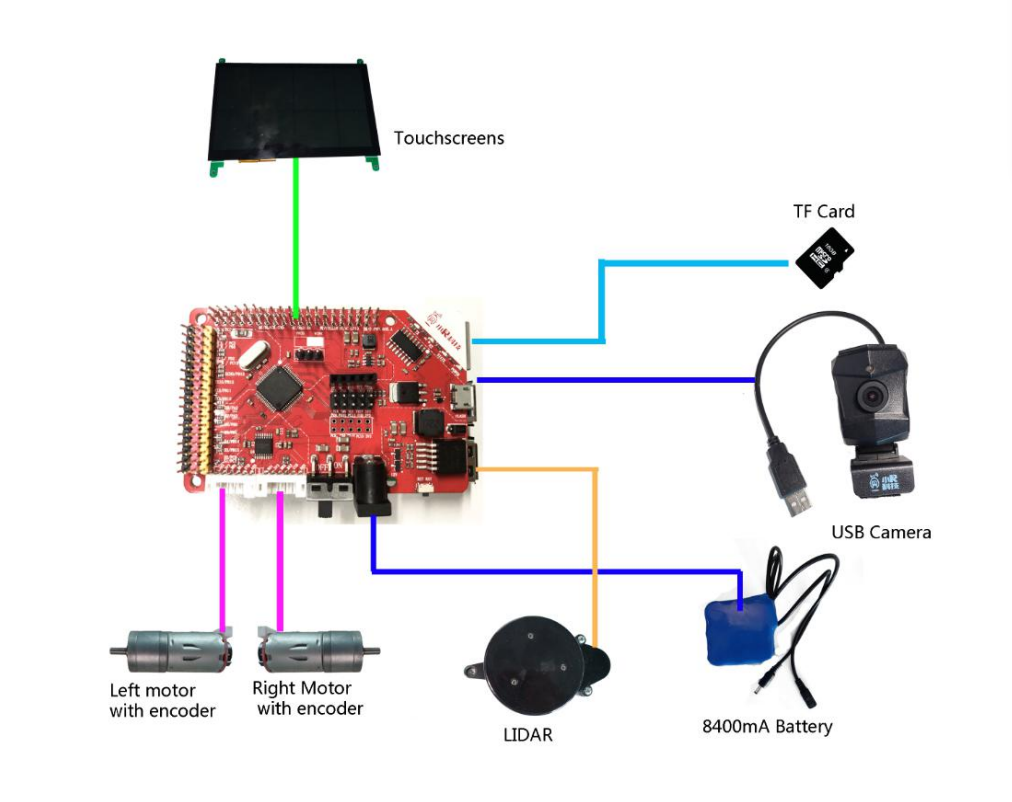
\includegraphics[width=5.2307in,height=4.4252in]{a0000-img016.png}}};
\end{scope}
\begin{scope}[xshift=5.824cm,yshift=-0.788cm]
\path[fill=white,even odd rule]  (NaN,NaN) --  (Infinity,NaN) --  (Infinity,-Infinity) --  (NaN,-Infinity) -- cycle;
\node[below,align=left,text width=NaNcm,transform shape] at (NaN,NaN) {\textcyrillic{Сенсорный экран}};
\end{scope}
\begin{scope}[xshift=11.164cm,yshift=-2.083cm]
\path[fill=white,even odd rule]  (NaN,NaN) --  (Infinity,NaN) --  (Infinity,-Infinity) --  (NaN,-Infinity) -- cycle;
\node[below,align=left,text width=NaNcm,transform shape] at (NaN,NaN) {\textcyrillic{Карта памяти}};
\end{scope}
\begin{scope}[xshift=12.539cm,yshift=-7.080cm]
\path[fill=white,even odd rule]  (NaN,NaN) --  (Infinity,NaN) --  (Infinity,-Infinity) --  (NaN,-Infinity) -- cycle;
\node[below,align=left,text width=NaNcm,transform shape] at (NaN,NaN) {USB-\textcyrillic{камера}};
\end{scope}
\begin{scope}[xshift=10.354cm,yshift=-10.456cm]
\path[fill=white,even odd rule]  (NaN,NaN) --  (Infinity,NaN) --  (Infinity,-Infinity) --  (NaN,-Infinity) -- cycle;
\node[below,align=left,text width=NaNcm,transform shape] at (NaN,NaN) {\textcyrillic{Аккумулятор, 8400 мА}};
\end{scope}
\begin{scope}[xshift=7.220cm,yshift=-10.478cm]
\path[fill=white,even odd rule]  (NaN,NaN) --  (Infinity,NaN) --  (Infinity,-Infinity) --  (NaN,-Infinity) -- cycle;
\node[below,align=left,text width=NaNcm,transform shape] at (NaN,NaN) {\textcyrillic{Лидар}};
\end{scope}
\begin{scope}[yshift=-9.738cm]
\path[fill=white,even odd rule]  (NaN,NaN) --  (Infinity,NaN) --  (Infinity,-Infinity) --  (NaN,-Infinity) -- cycle;
\node[below,align=center,text width=NaNcm,transform shape] at (NaN,NaN) {\textcyrillic{Левый и правый двигатели с
энкодерами}};
\end{scope}
\end{tikzpicture}


{\centering\itshape\color[HTML]{44546A}
Рисунок \stepcounter{qwerty}{\theqwerty}. Схема подключения платы управления приводами
\par}


\bigskip

PWR.ROS.A $\text{\textgreek{—}}$ это плата для управления приводами робота, соединяемая с платой
\foreignlanguage{english}{R}aspberry \foreignlanguage{english}{P}i 4B. Ее основные функции заключаются в следующем: 

\begin{enumerate}[series=listWWNumxxv,label=\arabic*.,ref=\arabic*]
\item Стабилизация напряжения: данная плата обеспечивает понижение входного напряжения 7–12\foreignlanguage{english}{ }В
постоянного тока до 5\foreignlanguage{english}{ }В или другого напряжения, которое требуется для питания основной платы
управления или приводов. 
\item Управление электродвигателями: данная плата обеспечивает управление приводами для движения робота вперед и назад,
остановки, ускорения, замедления.
\item Управление сервоприводами: данная плата оснащена 8-канальным выходным разъемом для подключения к сервоприводам.
При питании сервоприводов от платы последняя подходит для одновременного ШИМ-управления восемью сервоприводами с
напряжением питания 5 В и максимальным током не более 100 мА. 
\item Подключение датчиков: неиспользуемые разъемы GPIO на данной плате подключаются напрямую к плате
\foreignlanguage{english}{Raspberry} \foreignlanguage{english}{Pi} снизу (контакты обозначены желтым цветом).
\item Прием данных с датчиков, включая частоту вращения электродвигателя, показания гироскопа и другие основные
параметры.
\end{enumerate}

\bigskip

\subsection{Архитектура системы}
На следующей иллюстрации показана блок-схема работы алгоритма навигации.

\begin{tikzpicture}
\path (0,11.431) rectangle (14.950,0);
node[inner sep=0pt] at (7.475,5.716)
{\lfbox[margin=0mm,border-style=none,padding-top=0.0492in,padding-right=0.0984in,padding-bottom=0.0492in,padding-left=0.0984in]{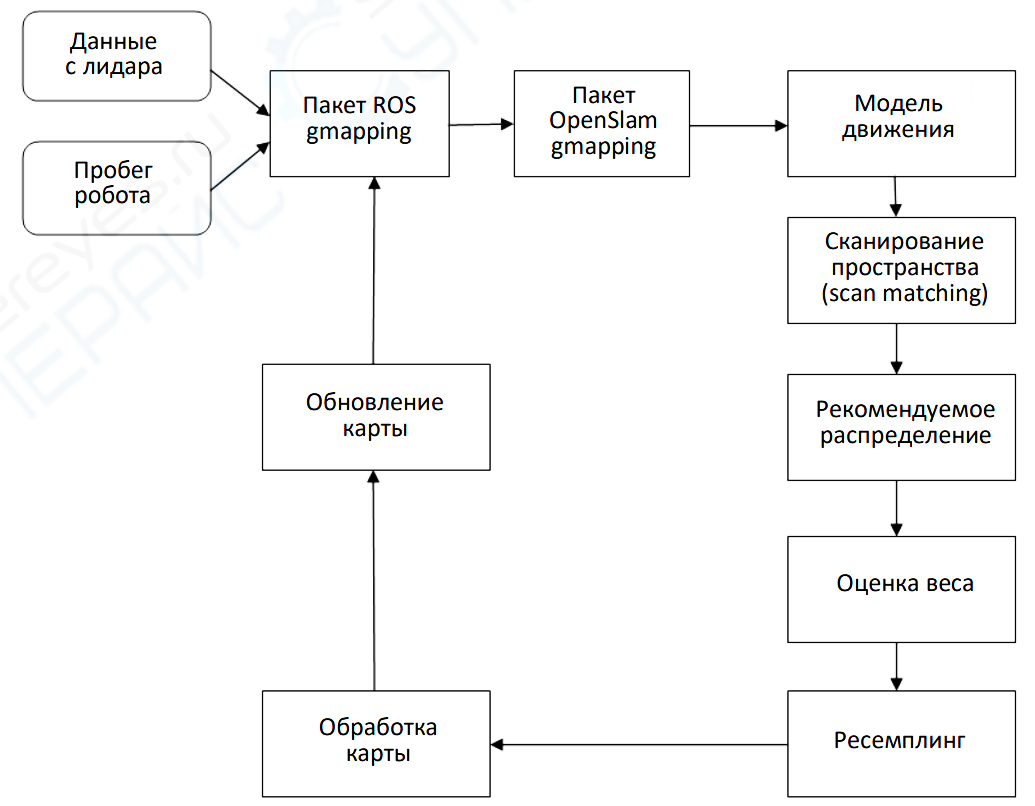
\includegraphics[width=5.8858in,height=4.5004in]{a0000-img017.png}}};
\begin{scope}[xshift=0.030cm,yshift=-3.388cm]
\path[fill=white,even odd rule]  (NaN,NaN) --  (Infinity,NaN) --  (Infinity,-Infinity) --  (NaN,-Infinity) -- cycle;
\end{scope}
\begin{scope}[xshift=3.732cm,yshift=-0.014cm]
\path[fill=white,even odd rule]  (NaN,NaN) --  (Infinity,NaN) --  (Infinity,-Infinity) --  (NaN,-Infinity) -- cycle;
\end{scope}
\end{tikzpicture}


{\centering\itshape\color[HTML]{44546A}
Рисунок \stepcounter{qwerty}{\theqwerty}. Архитектура системы
\par}

\clearpage\subsection[Описание алгоритма gmapping]{Описание алгоритма \foreignlanguage{english}{gmapping}}
Gmapping $\text{\textgreek{—}}$ это лазерный алгоритм SLAM, который был интегрирован в ROS, и это наиболее часто
используемый алгоритм SLAM среди мобильных роботов. Этот алгоритм был предложен Grisetti и др. в качестве метода SLAM
фильтрации частиц, основанного на Rao-Blackwellized. Алгоритм, основанный на фильтре частиц, использует множество
взвешенных частиц для представления апостериорной вероятности пути, и каждая частица предлагает важный фактор. Однако
для получения хороших результатов обычно требуется большое количество частиц, что увеличивает вычислительную сложность
алгоритма.

Процесс также снижает точность алгоритма. Проблема деградации частиц связана с удалением большого количества частиц из
набора образцов на этапе повторной выборки. Это произошло потому, что их важность может стать незначительной.
Следовательно, это означает, что существует определенная небольшая вероятность того, что правильная гипотетическая
частица будет исключена с течением времени. Чтобы избежать деградации частиц, был разработан метод адаптивной повторной
выборки.

Авторы также предлагают метод расчета точного распределения, учитывающего не только движение платформы робота, но и
недавние наблюдения. Предложенное распределение предлагается путем объединения наблюдаемых значений с диапазоном
движения. модель. Однако, когда мобильный робот оснащен очень точным датчиком LRF, можно использовать модель этого
датчика, поскольку она может достигать функций чрезвычайно высокого правдоподобия. На основе этого авторы интегрируют
недавние наблюдения датчика zt и вычисляют распределение Гаусса, чтобы приблизительно эффективно получить следующее
поколение распределения частиц.

Авторы интегрируют самое последнее наблюдение датчика 2. Кроме того, они вычисляют приближение Гаусса для эффективного
получения следующего поколения частиц. Параметры Гаусса


\lfbox[margin-right=0.0035in,margin-bottom=0.0035in,margin-top=0mm,margin-left=0mm,border-style=none,padding=0mm,vertical-align=top]{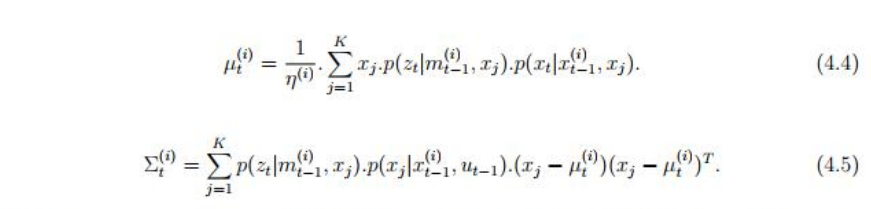
\includegraphics[width=6.4965in,height=1.5591in]{a0000-img018.png}}


Авторы интегрируют самое последнее наблюдение датчика 2. Кроме того, они вычисляют приближение Гаусса для эффективного
получения следующего поколения частиц. Параметры Гаусса


\lfbox[margin-right=0.0035in,margin-bottom=0.0083in,margin-top=0mm,margin-left=0mm,border-style=none,padding=0mm,vertical-align=top]{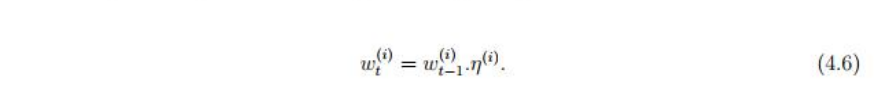
\includegraphics[width=6.4965in,height=0.7in]{a0000-img019.png}}


Где K $\text{\textgreek{—}}$ количество точек выборки, а µ $\text{\textgreek{—}}$ нормализованный коэффициент. Используя
это распределение, вес i-й частицы определяется как:


\lfbox[margin-right=0.0035in,margin-top=0mm,margin-bottom=0mm,margin-left=0mm,border-style=none,padding=0mm,vertical-align=top]{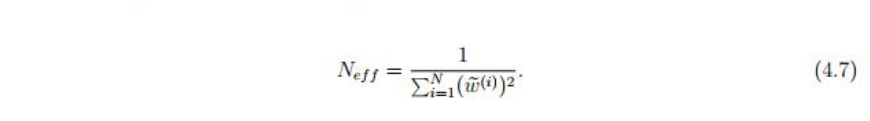
\includegraphics[width=6.4965in,height=0.9035in]{a0000-img020.png}}


Затем, используя (4.7), они вычисляют эффективное число N\foreignlanguage{english}{\textsubscript{eff}} частиц как
критерий, определяющий, когда следует выполнять шаг повторной выборки:

Эта адаптивная повторная выборка снижает неопределенность положения робота на этапах прогнозирования PF. В результате во
время процесса сопоставления сканирования требуется меньшее количество частиц из-за низкой неопределенности. В
экспериментах gmapping использовалось количество частиц 30, что очень мало по сравнению с обычным методом PF.
\end{document}
